\documentclass[]{spie}
\usepackage{geometry, mdwlist}                % See geometry.pdf to learn the layout options. There are lots.
\geometry{hmargin=1.5cm, vmargin=2cm}
\geometry{a4paper}                   % ... or a4paper or a5paper or ... 
%\geometry{landscape}                % Activate for for rotated page geometry
%\usepackage[parfill]{parskip}    % Activate to begin paragraphs with an empty line rather than an indent
\pagestyle{plain}
\usepackage[utf8]{inputenc} %accents under any OS but in TeXShop, requieres preferences/encoding to be set on UTF-8 BEFORE creating the document
\usepackage[greek,english,frenchb]{babel}
\usepackage{float}
\usepackage{subfigure}
\usepackage{hyperref}
\hypersetup{ 
     backref=true,    %permet d'ajouter des liens dans... 
     pagebackref=true,%...les bibliographies 
     hyperindex=true, %ajoute des liens dans les index. 
     colorlinks=true, %colorise les liens 
     breaklinks=true, %permet le retour à la ligne dans les liens trop longs 
     urlcolor= black,  %couleur des hyperliens 
     linkcolor= blue, %couleur des liens internes 
     bookmarks=true,  %créé des signets pour Acrobat 
     bookmarksopen=true,            %si les signets Acrobat sont créés, les afficher complètement. 
     citecolor=black,
} 

\usepackage{pdftricks}
\begin{psinputs}
   \usepackage{pstricks}
   \usepackage{pst-node}
\end{psinputs}

\usepackage{graphicx}
\usepackage{amssymb}
\usepackage{epstopdf}
\DeclareGraphicsRule{.tif}{png}{.png}{`convert #1 `dirname #1`/`basename #1 .tif`.png}

\pagestyle{empty} %Removes page numbers


%%%%%%%%%%%%%%%%%%%%%%%%%%%%%%%%%%%%%%%%%%%%%%%%%%%%%%%%%%%%%
\title{MetroloJ: an ImageJ plugin to help monitor microscopes' health.}
\author{Cédric Matthews$^{1,3}$ and Fabrice P. Cordelières$^{2,3}$
\skiplinehalf
$^{1}$CNRS-IBDML-UMR 6216, Service Imagerie, Marseille, France\\
$^{2}$Institut Curie/CNRS UMR 3348, PICT-IBiSA@Orsay, Orsay, France\\
$^{3}$Mission Ressources et Compétences Technologiques du CNRS, UPS 2274, Meudon, France}

%\date{}                                           % Activate to display a given date or no date

\begin{document}


\maketitle
%%%%%%%%%%%%%%%%%%%%%%%%%%%%%%%%%%%%%%%%%%%%%%%%%%%%%%%%%%%%
\begin{abstract}

Acquiring a good image requires having access to a well characterized, well calibrated imaging system. In this matter, procedures exist, aimed at measuring relevant parameters which helps testing, following and comparing microscopes performances. In this paper, we focus on four indicators: the estimation of the detector sensitivity , the evaluation of the field illumination homogeneity, the system resolution, and finally the characterization of its spectral registration. The built of reference samples and the subsequent image acquisition procedures are discussed. We introduce for the first time the MetroloJ plugin, designed to retrieve the four numerical indicators out of images, and to generate archivable reports as pdf files, thanks to the iText library. Altogether, the procedures and the MetroloJ plugin, already tested within the French technological network for multidimensional fluorescence microscopies (RT-MFM), provide the user with a mean to keep track of microscopes' health, and make it a valuable tool in choosing a microscope setup, based on pre-defined expectations.

\end{abstract}
%%%%%%%%%%%%%%%%%%%%%%%%%%%%%%%%%%%%%%%%%%%%%%%%%%%%%%%%%%%%
\keywords{Metrology, microscope calibration, image analysis, fluorescence microscopy.}

%%%%%%%%%%%%%%%%%%%%%%%%%%%%%%%%%%%%%%%%%%%%%%%%%%%%%%%%%%%%%
\section{Introduction}
\label{sec:intro}

MetroloJ was developed in order to keep track of the microscopes' health, allowing to get an archivable, well formatted report containing all measurements automatically done.
In this matter, it helps retrieve four indicators out of images generated using standardized procedures. Firstly, the performances of detectors might be compared using the coefficient of variation which estimates the detection associated noise. Secondly, the field illumination homogeneity is evaluated from a single image, using intensity profiles along the four axis passing through the image's center. Thirdly, the optical resolution might be extracted either from a 3D image of the PSF (Point Spread Function, allows extracting the x, y and z resolutions) or out of a XZ reflection view (lateral resolution only). Finally, misalignment within the optical system and/or chromatic aberration is evaluated from 3D multi-labelled beads images.\\
For each measurement, a plugin has been written, allowing generation of both a pdf file aimed at archiving the system's evaluation, and optionally of images and data tables for further processing. The former is generated by using an external library, iText (\href{http://itextpdf.com/}{http://itextpdf.com/}), which should be installed in order to use the MetroloJ plugin collection. All plugins' output are formatted in a similar way:
\begin{enumerate*}
	\item A visual representation of the original dataset either raw or modified view;
	\item Microscope infos: summarizes informations about the acquisition system and the image's calibration;
	\item Report specific sections;
	\item Sample infos (optional): user entered informations under the ``Sample infos'' section of the plugin interface;
	\item Comments (optional): user entered informations under the ``Comments'' section of the plugin interface.
\end{enumerate*}

%%%%%%%%%%%%%%%%%%%%%%%%%%%%%%%%%%%%%%%%%%%%%%%%%%%%%%%%%%%%%
\section{The MetroloJ plugins collection}
\label{sec:pgCollec}

%--------------------------------------------------------------------------------------------------------------------------------------------------------------------
\subsection{Generate CV report}
\label{subsec:gcvr}

\subsubsection*{Introduction}
\label{subsubsec:gcvr-intro}

The coefficient of variation (CV) is an indicator of the sensitivity of a detector. It is calculated by measuring both the average intensity ($\mu$) and the standard deviation ($\sigma$) of the gray levels on an image of a uniformly labeled fluorescent sample. As a reference sample, one could use either fluorescent plastic slides or preparations made of large fluorescent bead (see the material and methods section from Zucker 2006\cite{Zucker2006}). The CV corresponds to the ratio $\sigma/\mu$ which reflects, in a normalized way, the spread of the image's histogram. CV might be used either to compare several detectors such as photomultiplier tubes (PMTs) by keeping their specific settings (gain/offset) constant while acquiring the images, or compare several modes of function of a single detector (ex: sensitivity as a function of the PMT gain or as a function of the scanning averaging, see Zucker, 2006\cite{Zucker2006}). The lower the CV, the more sensitive the detector will be.

\subsubsection*{How does the plugin work ?}
\label{subsubsec:gcvr-pgWork}

The plugin measures the average intensity ($\mu$) and the standard deviation ($\sigma$) of the gray levels within a user defined region of interest (ROI). This procedure is repeated over each slice of the input stack, each one containing an acquisition made either with a detector or using parameters to test. It calculates the coefficient of variation as follows: $CV = \sigma/\mu$. The normalized CV is then calculated as the ratio of the current image's CV over the minimum retrieved CV over all images.

\subsubsection{What's on the report ?}
\label{sec:gcvr-report}

The CV report is composed of two pages (see an example of report on fig. \ref{fig:gcvr-report}) based on the user provided informations. It is composed of up to 6 sections:
\begin{figure}[h]
		\begin{center}
		\begin{tabular}{c}
			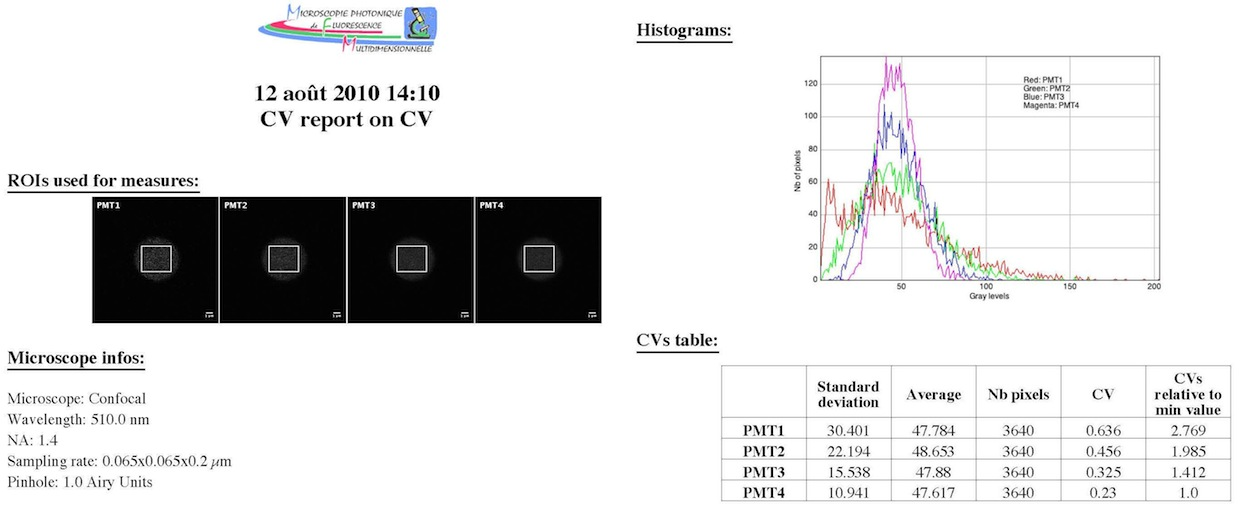
\includegraphics[width=0.95\linewidth]{img/gcvr-report}
		\end{tabular}
	\end{center}
	\caption{\label{fig:gcvr-report}Generate CV report: an example of report.}
\end{figure} 
\begin{itemize*}
	\item \textbf{\textit{ROIs used for measures}}: montage made from the input images, overlaid with the user defined ROIs;
	\item \textbf{\textit{Histograms}}: plot of the gray level distributions within the user defined ROIs;
	\item \textbf{\textit{CVs table}}: contains for each image the $\mu$ and $\sigma$ values, the ROI size (expressed in number of pixels), the raw and normalized CVs.
\end{itemize*}



%--------------------------------------------------------------------------------------------------------------------------------------------------------------------
\subsection{Generate field illumination report}
\label{subsec:gfir}

\subsubsection*{Introduction}
\label{subsubsec:gfir-intro}

As most of the images obtained from a microscope will be used either for topological information display or intensity quantification, estimating the illumination homogeneity is a process required for image quality assessment and further corrections. A quantification of this homogeneity might be obtained out of images made from a uniformly labelled sample such as a fluorescent plastic slide or a highly packed fluorescent beads preparation. Intensity profiles are to be made in order to estimate loss of intensity encountered at the image's border, and to evaluate the illumination centering accuracy relative to the field of view. Besides collecting information on the illumination field characteristics, it also helps get a diagnostic on problems such as presence of a dirty lens or a misalignment within the optical path (see Zucker and Price, 1999\cite{Zucker1999} for examples).


\subsubsection*{How does the plugin work ?}
\label{subsubsec:gfir-pgWork}

The plugin generates a normalized view of the image. Its maximum intensity pixel being set to 100\%, an iso-intensity map is drawn (original idea from Zucker and Price, 1999\cite{Zucker1999}). The coordinates from the maximum intensity pixel, the image barycenter and the from the 100\% region are retrieved. From the input image, the plugin will generate and analyze four intensity profiles along the horizontal, the vertical axis and both diagonals passing through the image's center. Raw and normalized intensities of 8 characteristic pixels, corresponding to the 8 intercepts of those lines are determined.

\subsubsection*{What's on the report ?}
\label{subsubsec:gfir-report}

The field illumination report is composed of two pages (see an example of report on fig. \ref{fig:gfir-report}) based on the user provided informations. It is composed of up to 6 sections:
\begin{figure}[h]
		\begin{center}
		\begin{tabular}{c}
			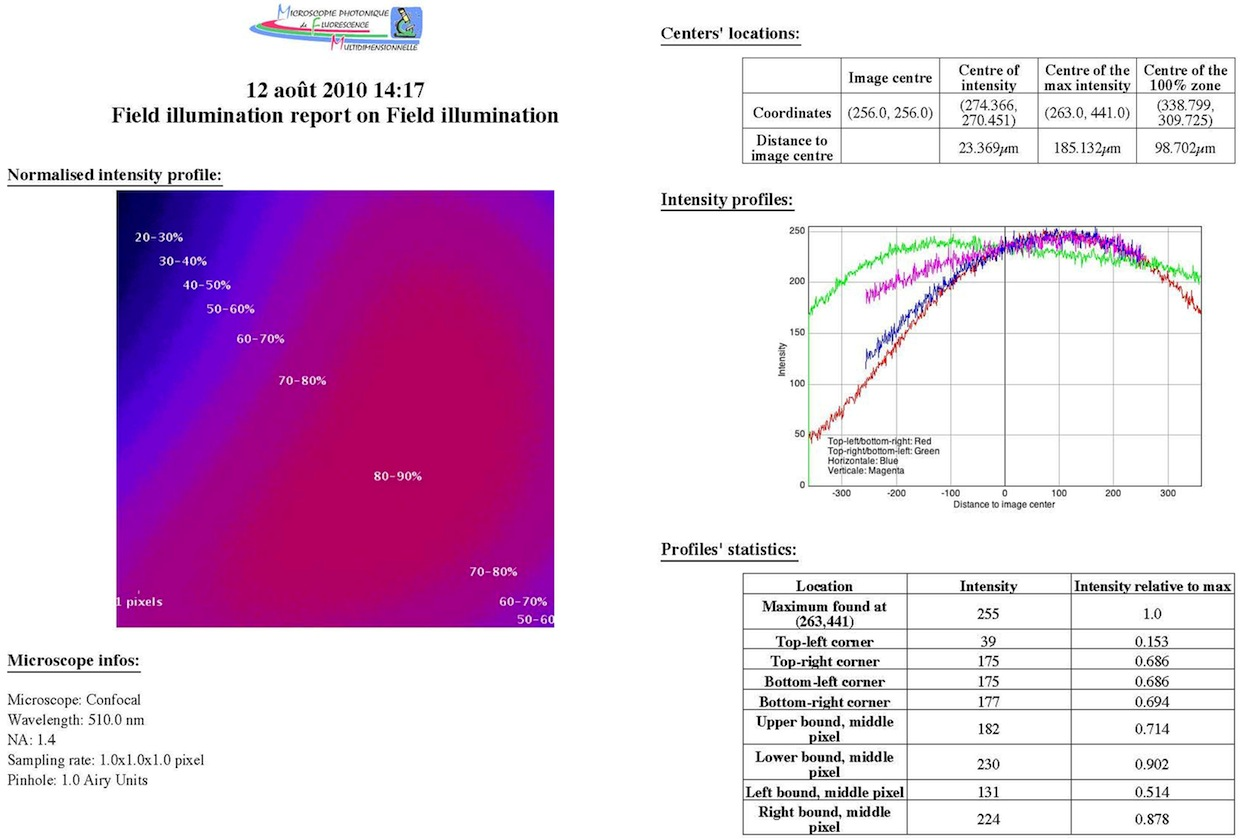
\includegraphics[width=0.9\linewidth]{img/gfir-report}
		\end{tabular}
	\end{center}
	\caption{\label{fig:gfir-report}Generate field illumination report: an example of report.}
\end{figure} 
\begin{itemize*}
	\item \textbf{\textit{Normalized intensity profile}}: normalized view of the field illumination, in false color, separated into iso-intensity zones which step width is user defined;
	\item \textbf{\textit{Centers' location}}: coordinates of 4 points of interest: the image center, the centre of intensity, the center of maximum intensity and the centre of the 100\% zone. It also displays the distances between the 3 later and the image's geometrical center;
	\item \textbf{\textit{Intensity profiles}}: a plot of the intensity profiles along the the horizontal, the vertical axis and both diagonals passing through the image's center;
	\item \textbf{\textit{Profiles' statistics}}: contains both raw and normalized intensities of 8 characteristic pixels, corresponding to the 8 intercepts of the lines along which the intensity profiles are retrieved.
\end{itemize*}

%--------------------------------------------------------------------------------------------------------------------------------------------------------------------
\subsection{Generate PSF report}
\label{subsec:gpr}

\subsubsection*{Introduction}
\label{subsubsec:gpr-intro}

The Point Spread Function (PSF) of a system gives a view of the modifications an optical system makes to the perception one has from a object seen through it. It can be recorded using a fluorescent sample of dimensions chosen below the expected resolution of the system (ex: preparations of small fluorescent beads). As the obtained pattern will be diffraction limited, its dimensions gives a measure of the optical resolution of the system. Intensity profiles made through the maximum intensity pixels of the image in all 3 dimensions might be fitted to a Gaussian (also this is not the most appropriate estimate of the PSF), its full width at half-maximum being a measure of the actual resolution of the system. Other analysis might be done on the PSF image, giving more detailed informations on the performances of the optical system. Those measures being beyond the scope of the paper, the reader might refer to Castaneda (1994)\cite{Castaneda1994} or Mahajan (1994)\cite{Mahajan1994} for more details.

\subsubsection*{How does the plugin work ?}
\label{subsubsec:gpr-pgWork}

The plugin generates a maximum intensity projection of the stack along the z axis. The (x, y) coordinates of the maximum intensity pixel (MIPix) are then collected. A XZ cross-section is generated from the original stack, along a line passing through the previously determined 2D MIPix. From this image, the z coordinate of the MIPix is extracted. The z slice is set to the z MIPix coordinate. The x profile and y profile are collected along the line passing through the MIPix. The z profile is collected on the XZ view, along the line passing through the MIPix. All three profiles are fitted to a Gaussian, using ImageJ's built-in curve fitting function. The resolution (FWHM) is calculated for each profile, based on the parameters retrieved from the fitting. The theoretical resolutions are calculated as follows, according to the microscope's type:
\begin{eqnarray}
	xy_{resol, wide-field}=\frac{0.61*\lambda_{emission}}{NA} \hspace{1cm} z_{resol, wide-field}=\frac{2*\lambda_{emission}}{NA^2}
	\label{eqn:gpr-WF}\\
	xy_{resol, confocal}=\frac{0.4*\lambda_{emission}}{NA} \hspace{1cm} z_{resol, confocal}=\frac{1.4*\lambda_{emission}}{NA^2}
	\label{eqn:gpr-conf}
\end{eqnarray}


\subsubsection*{What's on the report ?}
\label{subsubsec:gpr-report}

The PSF report is composed of two to three pages (see an example of report on fig. \ref{fig:gpr-report}) depending on the user provided informations. It is composed of up to 8 sections:
\begin{figure}[h]
		\begin{center}
		\begin{tabular}{c}
			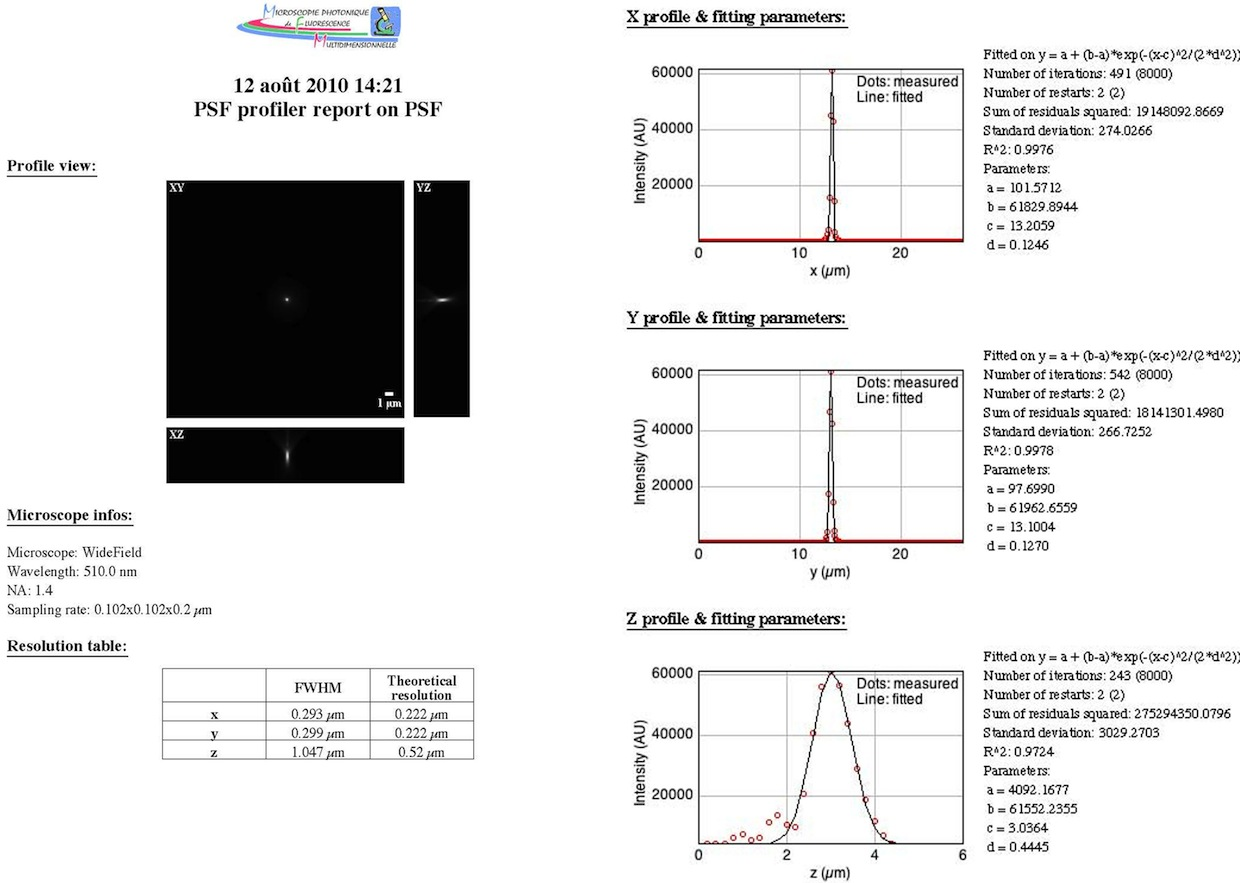
\includegraphics[width=0.9\linewidth]{img/gpr-report}
		\end{tabular}
	\end{center}
	\caption{\label{fig:gpr-report}Generate PSF report: an example of report.}
\end{figure} 
\begin{itemize*}
	\item \textbf{\textit{Profile view}}: montage made from the three maximum intensity projections, XY, XZ and YZ;
	\item \textbf{\textit{Resolution table}}: carries both the resolutions determined by fitting and the theoretical ones;
	\item \textbf{\textit{x, y, z profiles and fitting parameters}}: plots of the intensity profile along the x, y and z axis and the corresponding fitted curves. On the right side of the each graph stand the fitting parameters.
\end{itemize*}

%--------------------------------------------------------------------------------------------------------------------------------------------------------------------
\subsection{Generate axial resolution report}
\label{subsec:gaar}

\subsubsection*{Introduction}
\label{subsubsec:gaar-intro}

An alternative way to PSF recording to measure the axial resolution is to use a single reflecting mirror as a sample. Acquiring an XZ transversal imageallows visualizing interference fringes. Focussing on the widest one and fitting it to a Gaussian enables extraction of the axial resolution in the form of its FWHM (see Zucker, 2004\cite{Zucker2004}). To the difference of PSF analysis which measures the resolution on the emission path, the axial resolution is evaluated using only the excitation light.

\subsubsection*{How does the plugin work ?}
\label{subsubsec:gaar-report}

After the user has defined a rectangular ROI, the plugin will generate an average intensity projection of the image along the y axis. The resulting 1D intensity profile is then fitted to a Gaussian, using ImageJ's built-in curve fitting function. The axial resolution (FWHM) is calculated for each profile, based on the parameters retrieved from the fitting. The theoretical resolutions are calculated as already stated in equations \ref{eqn:gpr-WF} and \ref{eqn:gpr-conf}.

\subsubsection*{What's on the report ?}
\label{subsubsec:gaar-report}

The axial resolution report is composed of two pages (see an example of report on fig. \ref{fig:garr-report}). It is composed of up to 6 sections:
\begin{figure}[h]
		\begin{center}
		\begin{tabular}{c}
			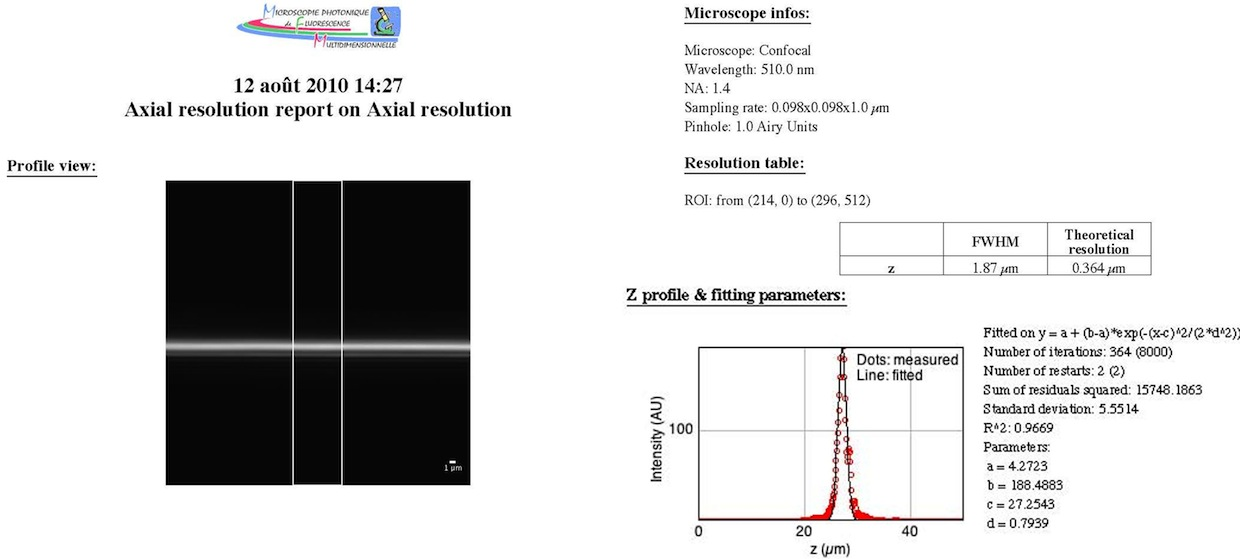
\includegraphics[width=0.9\linewidth]{img/garr-report}
		\end{tabular}
	\end{center}
	\caption{\label{fig:garr-report}Generate axial resolution report: an example of report.}
\end{figure} 
\begin{itemize*}
	\item \textbf{\textit{Profile view}}: input image overlaid by the user defined ROI;
	\item \textbf{\textit{Resolution table}}: carries both the ROI's position, as well as axial resolutions (experimental and theoretical);
	\item \textbf{\textit{z profile and fitting parameters}}: plot of the intensity profile along the z axis and the fitted curve. On the right side of the graph stand the fitting parameters.
\end{itemize*}

%--------------------------------------------------------------------------------------------------------------------------------------------------------------------
\subsection{Generate co-alignement report}
\label{subsec:gcoar}

\subsubsection*{Introduction}
\label{subsubsec:gcoar-intro}

The spectral registration over up to 4 channels is one argument manufacturer use for selling highly priced objectives. However, in real biological samples, two co-localizing signals might be captured well apart one from the other, generally as a consequence of misalignment within the optical path or from high refractive index mismatches within the sample. In any situation, this mis-registration/chromatic aberration should be quantified and images should be corrected, if possible, prior to further analysis. The sample of choice for such measurements consists of multi-labelled fluorescent beads, one 3D stack being recorded per channel. The center of mass for each channel might be calculated and the distances between centers estimated. Alternative methods exists, aiming at quantify the axial spectral registration, using a mirror slide and a procedure similar to the one described under section \ref{subsubsec:gaar-intro} (see Zucker, 2006\cite{Zucker2006}).

\subsubsection*{How does the plugin work ?}
\label{subsubsec:gcoar-pgWork}

The plugin will generate two summed intensity projections of the stack along the y and z axes. On each projection, histogram segmentation is done on the log of intensities, aiming at separating two populations of intensities (background and signal). Each projection is thresholded to highlight the ``signal pixels' population''. An ellipse is fitted to those pixels (i.e. to the bead's outline), and the coordinates of its centre of mass is determined. The full coordinates set is used to calculate center to center distances between all possible combinations of channels couples. For each couple, a reference distance $r_{ref}$ is calculated , taking into account the disparate resolutions over the three dimensions (see Cordelières and Bolte, 2008\cite{Cordelieres2008} for more details).

\subsubsection*{What's on the report ?}
\label{subsubsec:gcoar-report}

The co-alignement report is composed of two to three pages (see an example of report on fig. \ref{fig:gcoar-report}) depending on the user provided informations. It is composed of up to 7 sections:
\begin{figure}[h]
		\begin{center}
		\begin{tabular}{c}
			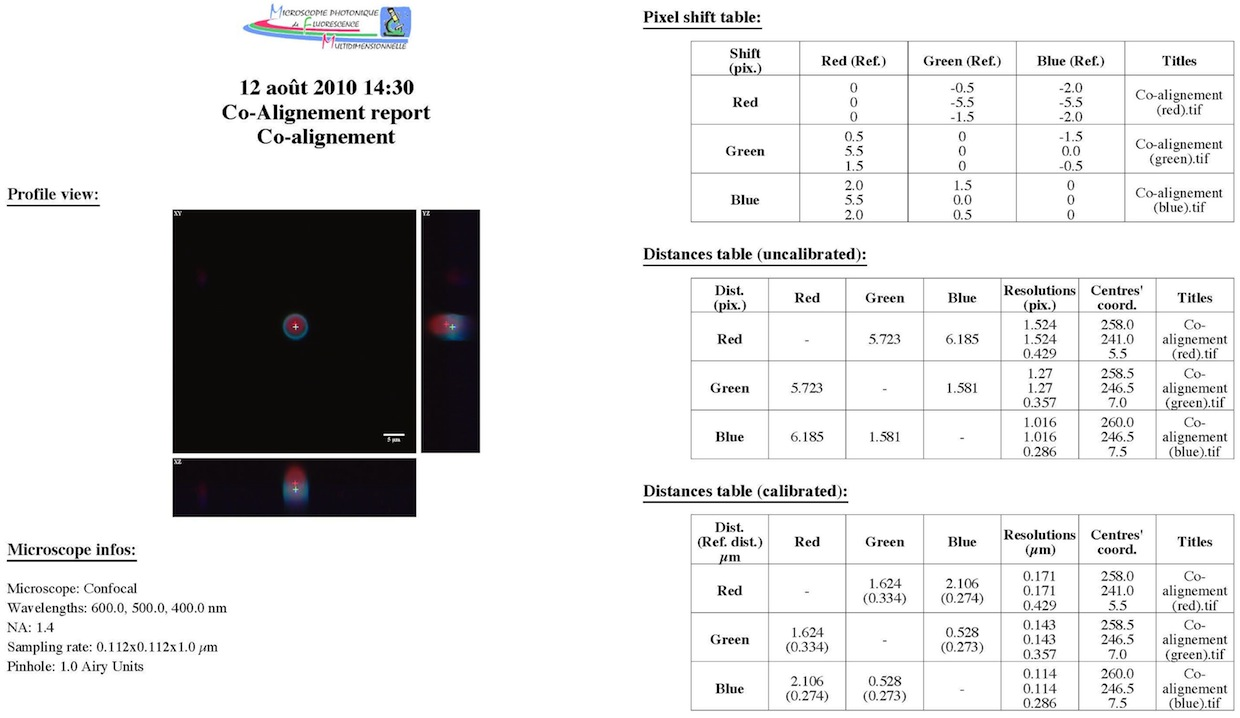
\includegraphics[width=0.9\linewidth]{img/gcoar-report}
		\end{tabular}
	\end{center}
	\caption{\label{fig:gcoar-report}Generate co-alignement report: an example of report.}
\end{figure} 
\begin{itemize*}
	\item \textbf{\textit{Profile view}}: montage composed of three maximum intensity projections, XY, XZ and YZ;
	\item \textbf{\textit{Pixel shift table}}: considering as a reference the channel stated at the beginning of each row, each column shows how much pixels separate one channel from the reference one along x, y and z axis. This information might be useful to compensate for chromatic aberration using image processing softwares. On each row, resolutions and centre's coordinates are given for the reference channel;
	\item \textbf{\textit{Distance table (uncalibrated)}}: contains distances calculated between two channels, while not taking into account the images' calibration;
	\item \textbf{\textit{Distance table (calibrated)}}: contains distances calculated between two channels, taking into account the images' calibration. The distance displayed between bracket is the reference distance (see \ref{subsubsec:gcoar-pgWork}).
\end{itemize*}

%%%%%%%%%%%%%%%%%%%%%%%%%%%%%%%%%%%%%%%%%%%%%%%%%%%%%%%%%%%%%
\section{Conclusions and future work}
\label{sec:concFut}

Altogether, the MetroloJ plugins collections allows quantifying four fundamental parameters evaluating the microscope's health: detector sensitivity, field illumination homogeneity, lateral and axial resolutions as well as 3D spectral registration. The output of the plugins, in the form of pdf files as well as spreadsheets, allow both archiving and further analysis of the results. Keeping track of the 4 parameters, one can easily foresee troubles arising on optical system and take action in order to correct them. The plugins collection might also be used in order to test a system prior to purchase. By the easiness of obtaining relevant images and the simplicity of use of the software package, one could confront the expected performances of a microscope to its actual specifications.\\
In the near future, we plan to link the MetroloJ package to a database in order to ease the archiving process. We also expect to collect enough data from the Imaging Facilities registered within the French technological network for multidimensional fluorescence microscopies (RT-MFM), in order to build a dynamic benchmarking system.


%%%%%%%%%%%%%%%%%%%%%%%%%%%%%%%%%%%%%%%%%%%%%%%%%%%%%%%%%%%%%
\acknowledgments
 
We would like to acknowledge the work of all the valuable beta-tester and the member of the ``groupe de travail Métrologie du RT-MFM'' who made feedback on the plugins collection and helped us improving and adapting it: Pierre Bourdoncle, Anne Cantereau, Julien Cau, Christophe Chamot, Julien Cianfichi, 
Aurélien Dauphin, Olivier Duc, Sylvain De Rossi, Stéphanie Dutertre, Aude Jobart-Malfait, Christophe Klein, Marc Lartaud, Patricia Le Baccon, Aurélie Le Ru, Meriem Garfa-Traoré, Camille Lebugle, Sandrine Leveque-Fort, Christophe Machu, Laure Malicieux, Christel Poujol, Richard Schwartzmann, Damien Schapman, Marie-Noëlle Soler, Nicolas Tissot, Yves Usson and Fran\c cois Waharte.


%%%%%%%%%%%%%%%%%%%%%%%%%%%%%%%%%%%%%%%%%%%%%%%%%%%%%%%%%%%%%
\bibliography{ImageJ-MetroloJ}   %>>>> bibliography data in report.bib
\bibliographystyle{spiebib}   %>>>> makes bibtex use spiebib.bst


\end{document}  